\section{Continuous Training and Serving} \label{continuous-training-serving}
In this section, we describe how we take advantage of the properties of SGD to implement our proactive training, online statistics computation, and feature materialization.
Another important aspect of any deployment platform is the ability to monitor the quality of the deployed model.
We present our method for evaluating the quality of the deployed model and how we guarantee high-quality models.
Finally, we describe how our continuous training approach improves the efficiency of the deployment process.
\subsection{Proactive Training} \label{proactive-training}
Proactive training replaces the periodical offline retraining of the deployed model.
In periodical training, the deployment platform is reactive and retrains a new model when the quality drops below a user defined threshold or a large amount of training data becomes available.
In proactive training, we constantly train the deployed model using the incoming and existing historical data.

We use the iterative nature of SGD in the design of the proactive training.
The input to each iteration of SGD is the current weights of the model, one or more data points, and an objective function.
In proactive training, we execute iterations of SGD on the deployed model.
The deployment platform, first samples the historical data, then transforms the data using the deployed pipeline.
Next, the proactive trainer uses the resulting data to compute the gradient of the objective function and finally update the deployed model.

The two parameters of SGD (learning rate and sample size) play an important role in proactive training.
They have to be tuned to increase the efficiency of the training.
Choosing  a very small sample size may result in inaccurate updates and as a result, degrade the quality of the deployed model.
On the other hand, a very large sample size leads to a lengthy training process and less frequent model updates.
Similarly, learning rate should be adapted accordingly.
The process of choosing the best sample size and learning rate adaptation technique is similar to static training.
Different hyperparameter tuning techniques are proposed for finding the best set of hyperparameters.
Most common and simplest approaches are grid search and random search \cite{bergstra2012random}.
We use a grid search over the initial training data to find the best hyperparameters (in our system, learning rate adaptation technique and sample size).
Once the initial model is trained and deployed, the same set of parameters are used for the proactive training.
In deployment platforms, it is also possible that the distribution of the data changes overtime.
In Section \ref{evaluation}, we show that simple hyperparameter tuning methods result in the best set of parameters for the proactive training.
We also show that training a deployed model using the proactive training method results in a similar (or lower) error rate to the periodical retraining while using fewer resources.

The deployment platform should always adapt the deployed model to the more recent data items.
As a result, when sampling the historical data, one has to consider the effect of the sample on the deployed model.
A time-based sampling approach of the historical data emphasizes the more recent data points and better adopts the deployed model to the changes in the data distribution.
In Section \ref{evaluation}, we evaluate the performance of the deployed model using different sampling techniques (time-based, uniform, and window-based).

%\textit{Model Stability}
%To ensure that proactive training does not degrade the quality of the model, a model evaluator is used to assess the quality of the model.
%The proactive trainer uses the latest deployed model as an initial starting point and updates the model based on the training data.
%The evaluator assesses the quality of the model using an evaluation dataset or the prequential evaluation method \cite{dawid1984present}.
%If the quality of the model has degraded, the update is discard and the model is logged.
%This is to avoid over training the deployed model in proactive training.

%\todo[inline]{I'm going to remove scheduling rate and just run proactive training when the sample buffer is full}
%\textit{Scheduling rate.}
%\hl{An extra parameter of proactive training is the scheduling rate.
%In offline training, iterations of SGD are executed one after the other until convergence.
%In proactive training, the scheduling rate defines the frequency of SGD iteration execution.
%The scheduling rate plays an important role as it directly affects the freshness of the deployed model.
%However, a high scheduling rate results in many frequent SGD iterations which incur an overhead on the deployment system as it is using a lot of resources.
%A small scheduling rate also affects the model freshness.
%To increase the efficiency of the system a scheduler component is designed that is tasked with scheduling new iterations of SGD.
%Similar to learning rate tuning, we use an adaptive approach to adjust the scheduling rate.
%We describe a method for tuning the scheduling rate based on the rate of the incoming training data.
%The scheduling rate is increased as the rate of the incoming training data increases and vice versa.
%This helps in adapting the model to the new training data.}

\subsection{Online Statistics Computation and Feature Materialization}
Before updating the deployed model using the proactive training, the data has to be processed by the pipeline.
Some components of the machine learning pipeline, such as the standard scaler or the one-hot encoder, require statistics over the dataset to be calculated before they process the data.
Computing these statistics require scans of the data.
In our deployment platform, we utilize online training as well as proactive training.
During the online update of the deployed model, we compute all the necessary statistics for every component.
Computing the required statistics online eliminates the need to recompute the statistics for proactive training.

Moreover, during the online learning, the deployed pipeline transforms the incoming data to a set of features before updating the model.
Given enough storage space, our deployment platform first assigns timestamps and then caches these preprocessed features.
Therefore, while performing the proactive training, instead of sampling from the raw historical data, the deployment platform samples the features directly from the cache.
Caching the features completely eliminates the data preprocessing part of the pipeline during the proactive training and significantly reduces the total training time for the proactive training.

\textit{Dynamic model size.}
Depending on the type of the pipeline components, the size of the deployed model may need to be adjusted during the online or proactive training.
For example, one-hot encoding and data bucketization, both may generate new features after processing new training data.
After every statistics update, we analyze the changes made in the pipeline.
If any of the changes result in an increase in the model size, we dynamically adjust the model size in the next proactive training. 


\subsection{Improved Deployment Process}
\begin{figure*}[t]
\begin{subfigure}{\columnwidth}
\centering
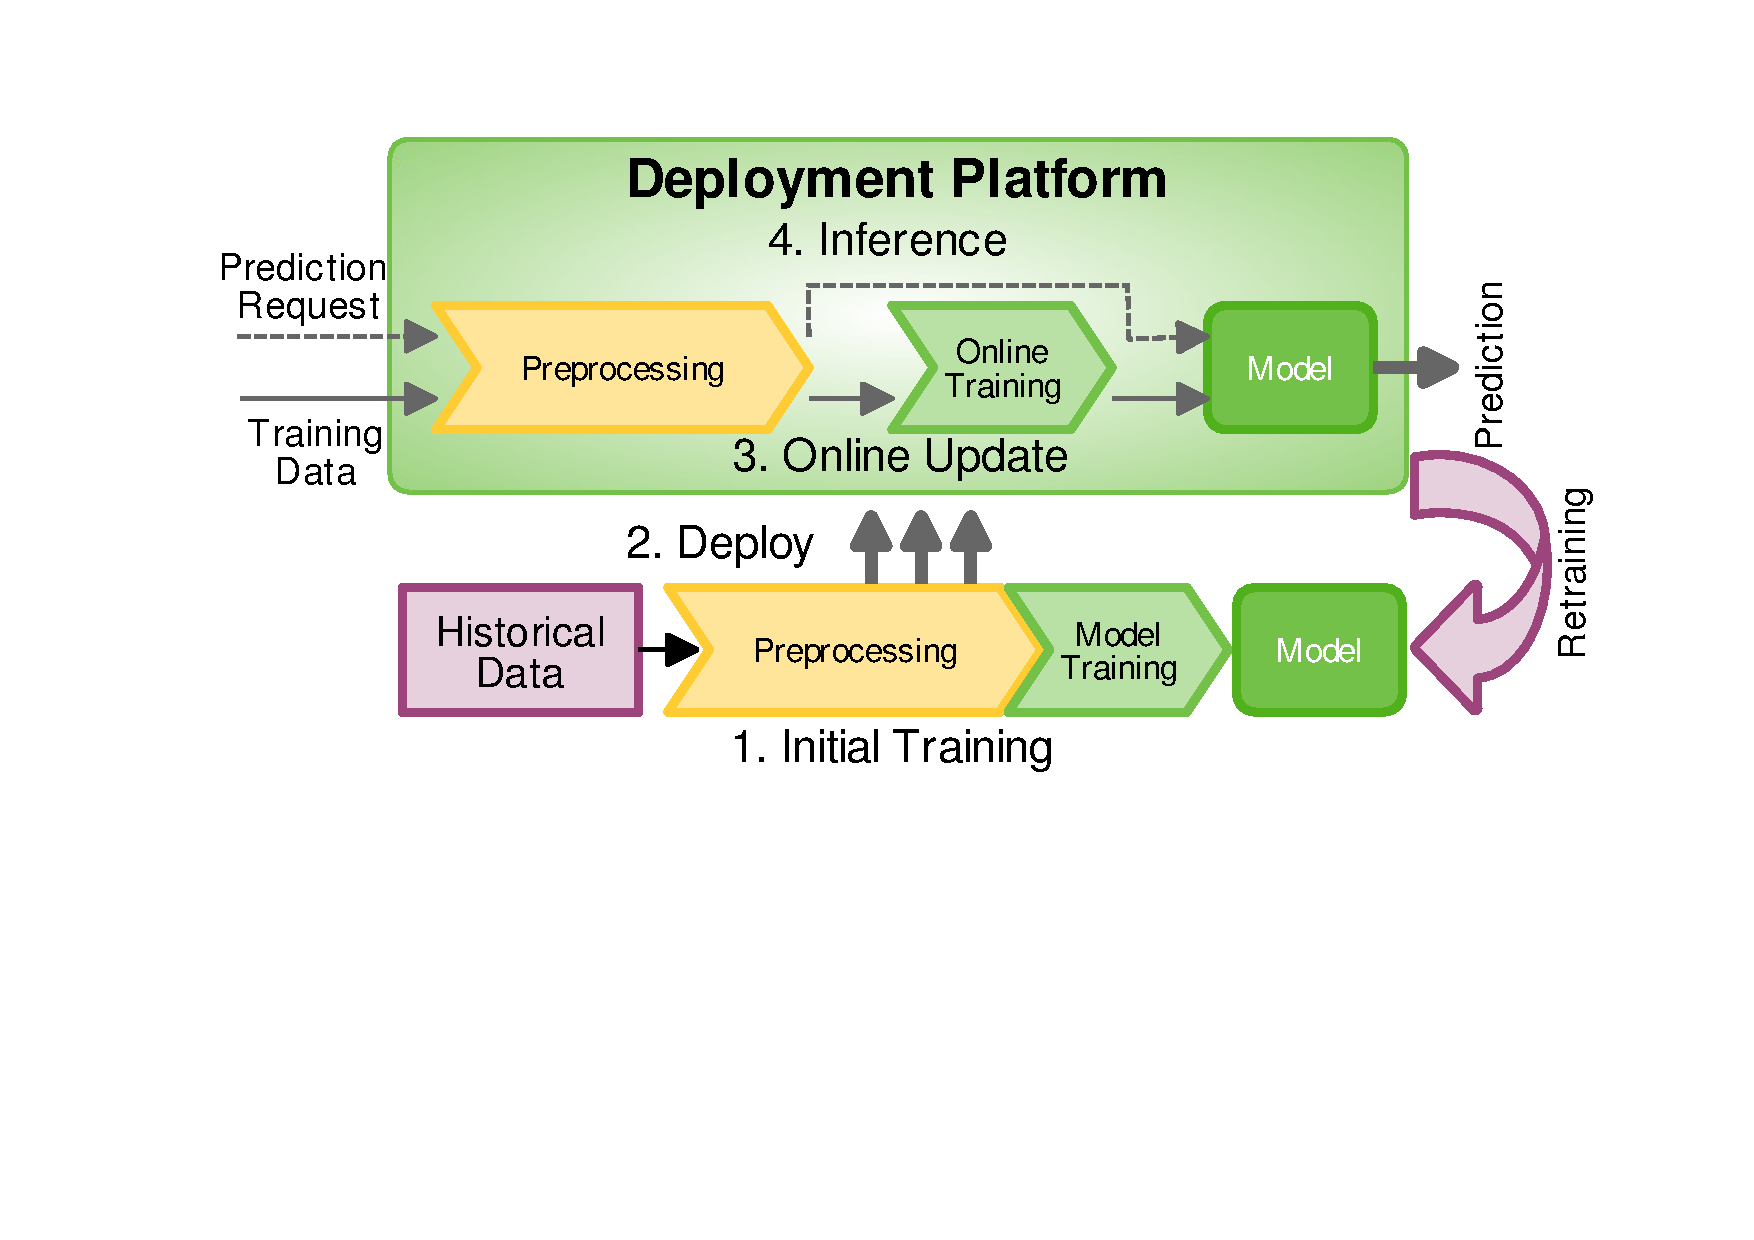
\includegraphics[width=\columnwidth]{../images/generic-motivational-example-v2.pdf}
\caption{Periodical deployment of machine learning pipelines}
\label{fig:motivational-example}
\end{subfigure}%
\begin{subfigure}{\columnwidth}
\centering
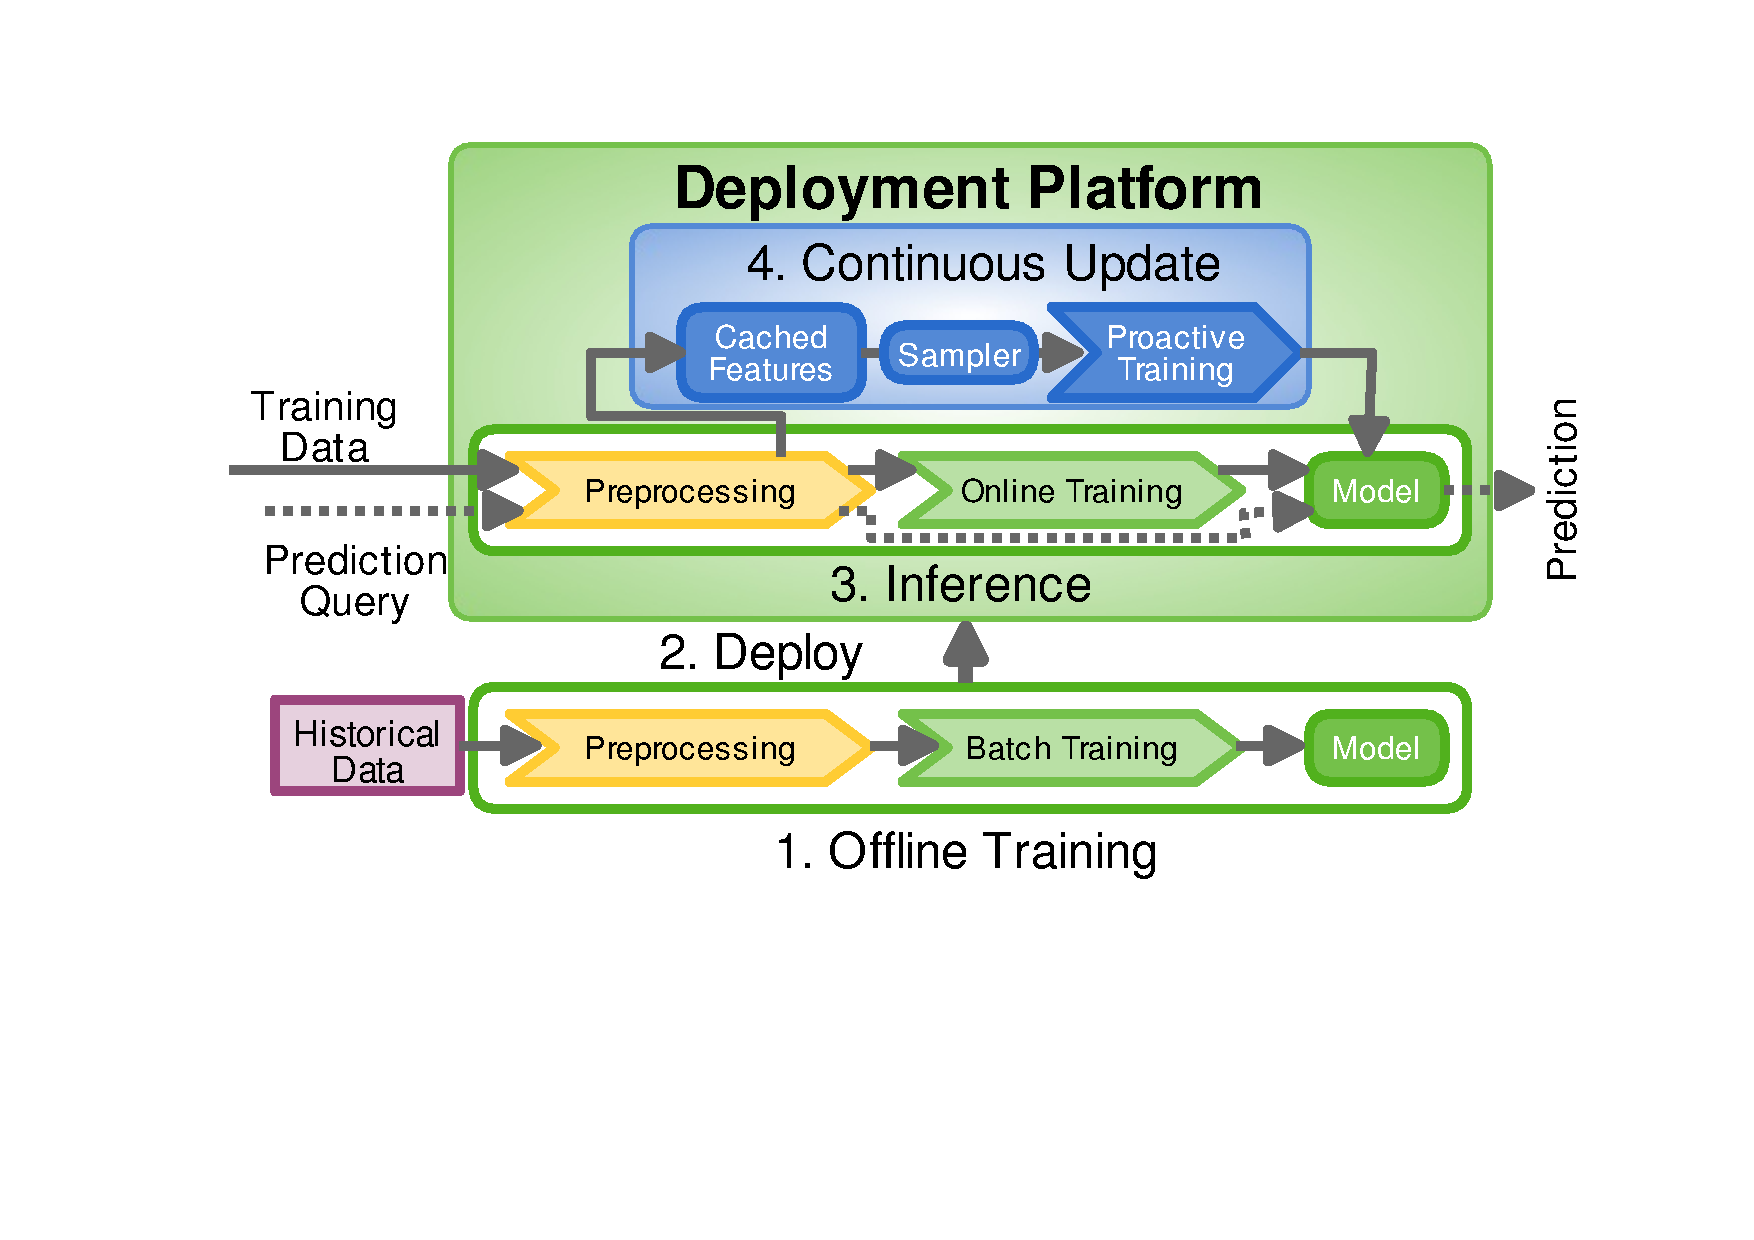
\includegraphics[width=\columnwidth]{../images/generic-improved-example-v2.pdf}
\caption{Continuous deployment of machine learning applications}
\label{fig:improved-example}
\end{subfigure}
\end{figure*}

Figure \ref{fig:motivational-example} shows the process of the periodical deployment approach.
During the initial training step, a user designs a machine learning pipeline that consists of several data and feature preprocessing steps and trains a machine learning model by utilizing a batch training algorithm.
Then in the deployment step, the model and the pipeline are deployed into the deployment platform.
To perform inference, the deployment platform directs the incoming prediction queries through the preprocessing steps.
Using the preprocessed features, the model makes a prediction.
During the online update phase, the deployment platform directs the data through the preprocessing steps of the pipeline and then, using an online training algorithm, the platform updates the model.
Finally, the deployment platform accommodates periodical retraining of the pipeline by either automatically initiating a batch training or prompting the user to train and redeploy a new model to the deployment platform.
During the periodical retraining, the deployment platform has to disable the online updating of the model.

Figure \ref{fig:improved-example} shows how our continuous training approach improves the existing deployment approach.
Similar to the current deployment process, a user first trains a pipeline and deploy it into the deployment platform.
The deployment platform uses the deployed pipeline and model to answer prediction queries and update the model using the incoming training data.
After the incoming training data are preprocessed, they are stored in a cache.
During the proactive training, samples of the features from the cache are used to compute a partial gradient.
The model is then updated using the computed gradient.
In the new workflow, the deployment platform continuously updates the pipeline and the deployed model without requiring a full retraining over historical data.
The deployment platform ensures that the model is always up-to-date.